\documentclass{beamer}

\usepackage{mathtools}
\usepackage{hyperref}
\usepackage{physics}
\usepackage{graphicx}
\usepackage{float}
\usepackage{subfigure}
\usepackage{color}
\usepackage{cite}
\usepackage[numbers]{gbt7714}
\usepackage{indentfirst}
\setlength{\parindent}{2em}
\usepackage{pifont}
\usepackage{comment}
\usepackage[orientation=landscape,size=custom,width=16,
height=9,scale=0.5,debug]{beamerposter}
\usepackage{wrapfig}
\hypersetup{pdfpagemode=FullScreen}
\usepackage{multicol}
\usepackage{amsmath,amssymb}
\usepackage{fontspec}
\usepackage{unicode-math}
\usepackage{listings}
\usepackage{algorithm}

\setmainfont{Times New Roman}
\setmathfont{XITS Math}


\title{Simulations with MPS/MPO}
\author{Kunyang DU}
\institute{Institue of Theoretical Physics}
\date{\today}

\begin{document}

\begin{frame}
	\titlepage
\end{frame}

\begin{frame}
	\frametitle{Model}
	\begin{itemize}
		\item \textbf{Hamiltonian:} Transverse Ising Model
		\begin{equation}
			H = -J\sum_{i=1}^{N-1}\sigma_i^z \sigma_{i+1}^z -h\sum_i^N\sigma_{i=1}^x + h_z\sum_{i=1}^N\sigma_i^z
		\end{equation}
		\item \textbf{Parameters} Physics parameters:
		\begin{equation}
			J = \pm 1.0,\quad h = 0.5,\quad N = 12
		\end{equation}
	\end{itemize}
\end{frame}

\begin{frame}
	\frametitle{Model:MPO}
	\begin{itemize}
		\item \textbf{Hamiltonian:} In kron form:
		\begin{equation}
			\begin{aligned}
				H = & J\sigma_1^z\otimes\sigma_2^z\otimes \mathbb{1}\otimes\mathbb{1}\otimes\cdots + \mathbb{1}\otimes J\sigma_2^z\otimes\sigma_3^z\otimes \mathbb{1}\otimes\cdots\\
				&+h\sigma_1^x\otimes\mathbb{1}\otimes\mathbb{1}\otimes\cdots + \mathbb{1}\otimes h\sigma_2^x\otimes\mathbb{1}\otimes\cdots \\
				& + h_z\sigma_1^z\otimes\mathbb{1}\otimes\mathbb{1}\otimes\cdots + \mathbb{1}\otimes h_z\sigma_2^z\otimes\mathbb{1}\otimes\cdots
			\end{aligned}
		\end{equation}
		\item \textbf{MPO} 
		\begin{equation}
			\begin{gathered}
				H_1 = \begin{pmatrix}
					h\sigma_1^x + h_z \sigma_1^z,& J\sigma_1^z,&\mathbb{1}
				\end{pmatrix},\\
				H_i = \begin{pmatrix}
					\mathbb{1},&\mathbb{0},&\mathbb{0}\\
					\sigma_i^z,&\mathbb{0},&\mathbb{0}\\
					h\sigma_i^x + h_z \sigma_i^z,& J\sigma_i^z,&\mathbb{1}
				\end{pmatrix},\quad 
				H_N = \begin{pmatrix}
					\mathbb{1}\\ \sigma_N^z\\h\sigma_N^x + h_z \sigma_N^z
				\end{pmatrix}
			\end{gathered}
		\end{equation}
	\end{itemize}
\end{frame}

\begin{frame}
	\frametitle{Model:MPO}
	\begin{itemize}
		\item \textbf{Total Magnetic Moment:} In kron form:
		\begin{equation}
			M_z =\sigma_1^z\otimes\mathbb{1}\otimes\mathbb{1}\otimes\cdots + \mathbb{1}\otimes \sigma_2^z\otimes\mathbb{1}\otimes\cdots
		\end{equation}
		\item \textbf{MPO} 
		\begin{equation}
			\begin{gathered}
				H_1 = \begin{pmatrix}
					\sigma_1^z,&\mathbb{1}
				\end{pmatrix},\\
				H_i = \begin{pmatrix}
					\mathbb{1},&\mathbb{0}\\
					\sigma_i^z,&\mathbb{1}\\
				\end{pmatrix},\quad 
				H_N = \begin{pmatrix}
					\mathbb{1}\\ \sigma_N^z
				\end{pmatrix}
			\end{gathered}
		\end{equation}
	\end{itemize}
\end{frame}

\begin{frame}
	\frametitle{Model:MPS}
	$\ket{s_i}$ denote that site $i$ is in eigenstate of $\sigma_i^z$ with eigenvalue$s_i=\pm 1$.\\
	$\ket{s_1s_2s_3\cdots s_N}$is corresponding many body basis of system.
	\begin{itemize}
		\item \textbf{Random Initialized State:} Random initial state
		\begin{equation}
			\psi_0 = \sum_{\{ s_i \}}C_{s_1s_2s_3\cdots s_N}\ket{s_1s_2s_3\cdots s_N}
		\end{equation}
		equals the random tensor $C_{s_1s_2s_3\cdots s_N}$. Then orientSVD:
	\end{itemize}
\end{frame}

\begin{frame}
	\frametitle{Model:MPS}
	\begin{itemize}
		\item \textbf{Assigned Initialized State} FM corresponds to state $C_{s_1s_2s_3\cdots s_N}$ with 
		\begin{equation}
			C_{111\cdots 1}=1\quad \text{or}\quad  C_{-1-1-1\cdots -1}=1
		\end{equation}
		while AFM corresponds to state $C_{s_1s_2s_3\cdots s_N}$ with 
		\begin{equation}
			C_{1-11-1\cdots}=1\quad \text{or}\quad  C_{-11-11\cdots}=1
		\end{equation}
		Then orientSVD in the same way as that in Random Initialized State.
	\end{itemize}
\end{frame}

\begin{frame}
	\frametitle{DMRG: 1-site update}
	\begin{multicols*}{2}
	\begin{itemize}
		\item Initialize MPS with diagonalization center at $i=1$.
		\begin{figure}[H]
			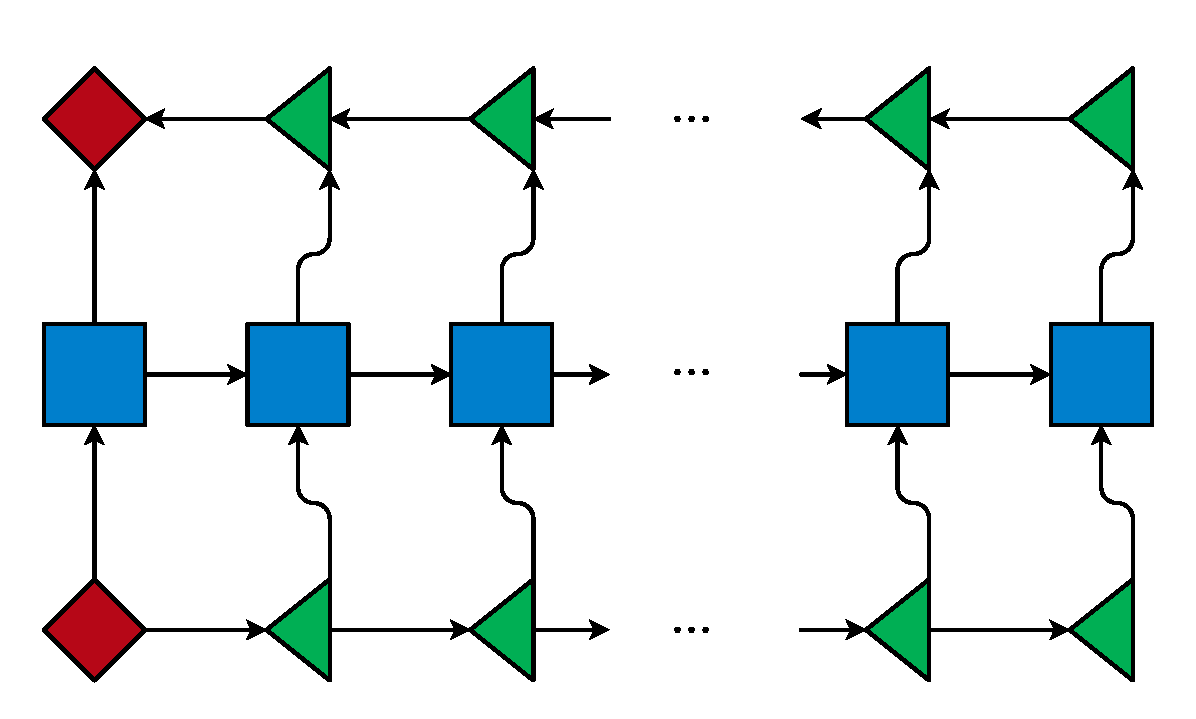
\includegraphics[width=1. \linewidth]{images/Initialization.pdf}
		\end{figure}
		\newpage
		\item Sweep at two direction (right - left - right - \dots)
		\begin{itemize}
			\item Calculate the left/right environment $H_L/H_R$.
			\begin{figure}[H]
				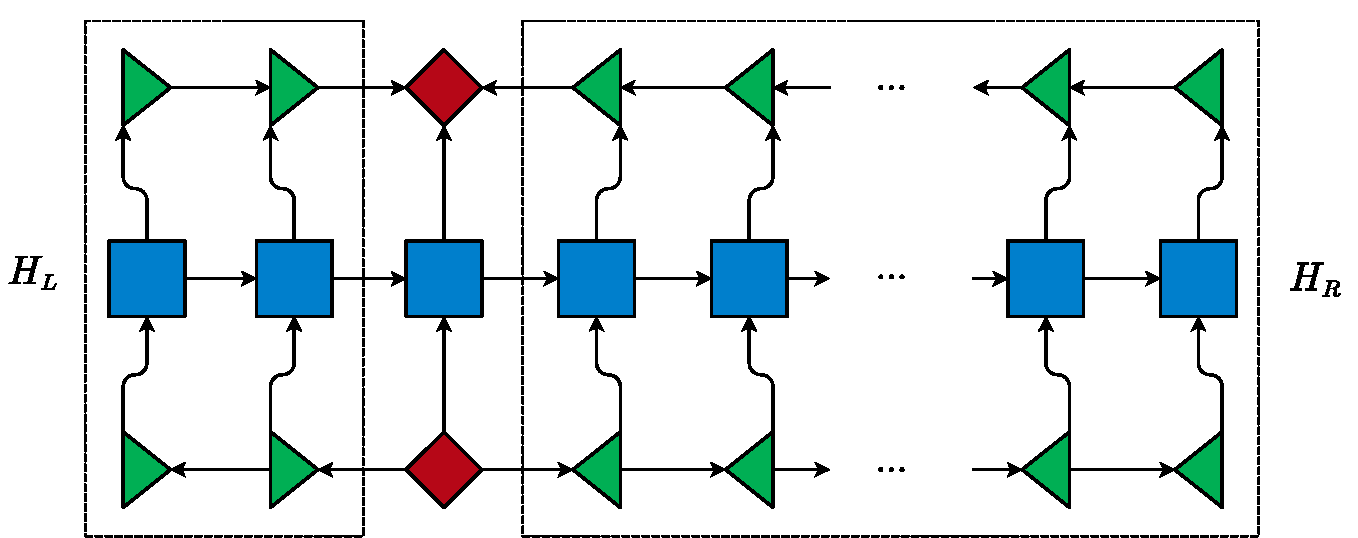
\includegraphics[width=1. \linewidth]{images/LRenv1.pdf}
			\end{figure}
		\end{itemize}
	\end{itemize}
	\end{multicols*}
\end{frame}

\begin{frame}
	\frametitle{DMRG: 1-site update}
	\begin{itemize}
		\item Sweep at two direction (right - left - right - \dots)
		\begin{itemize}
			\item Calculate the effective Hamiltonian $H_{eff} = H_L H_i H_R$
			\begin{figure}[H]
				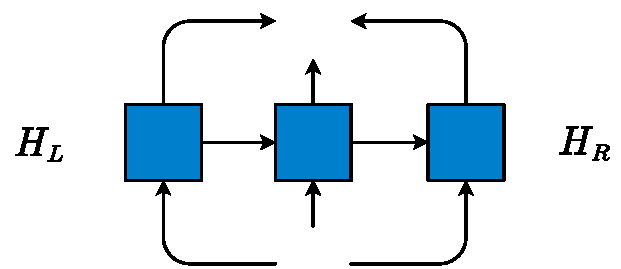
\includegraphics[width=0.3 \linewidth]{images/effH1.pdf}
			\end{figure}
			\item OrientSVD and move the center to next site.
			\begin{figure}[H]
				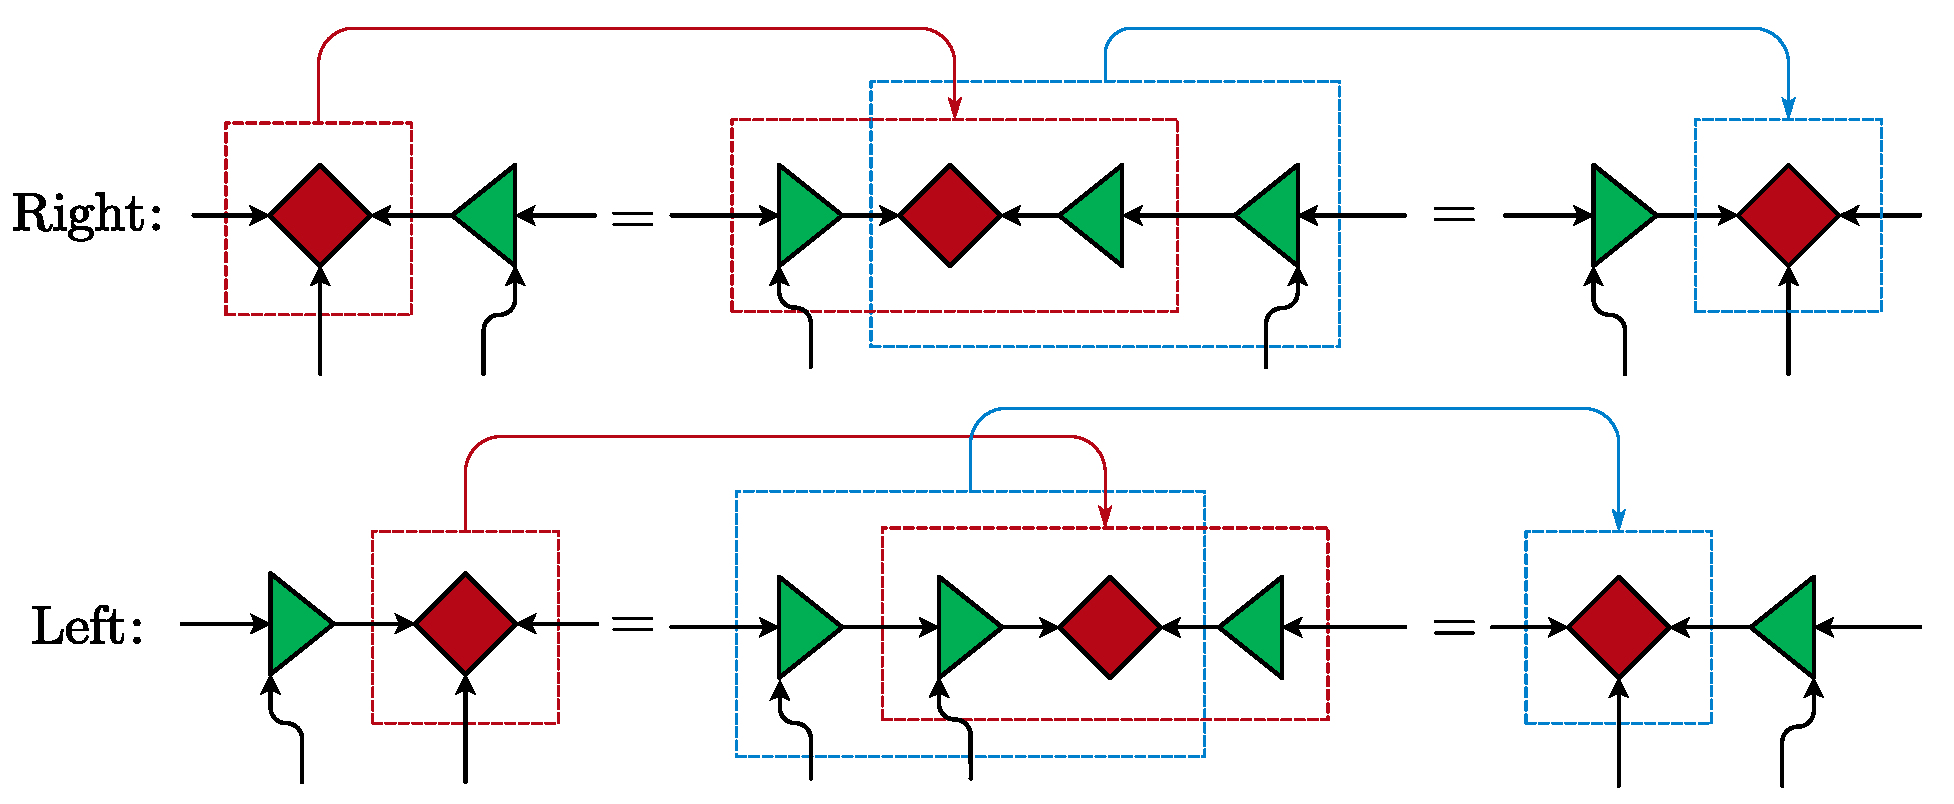
\includegraphics[width=0.6 \linewidth]{images/orientSVD.pdf}
			\end{figure}
		\end{itemize}
	\end{itemize}
\end{frame}


\begin{frame}
	\frametitle{TDVP: 1-site integration}
	\begin{itemize}
		\item Initialize MPS with diagonalization center at $i=1$.
		\newpage
		\item Sweep at two direction (right - left - right - \dots)
		\begin{itemize}
			\item Calculate the left/right environment $H_L(t+\Delta t/2)/H_R(t)$.
			\begin{figure}[H]
				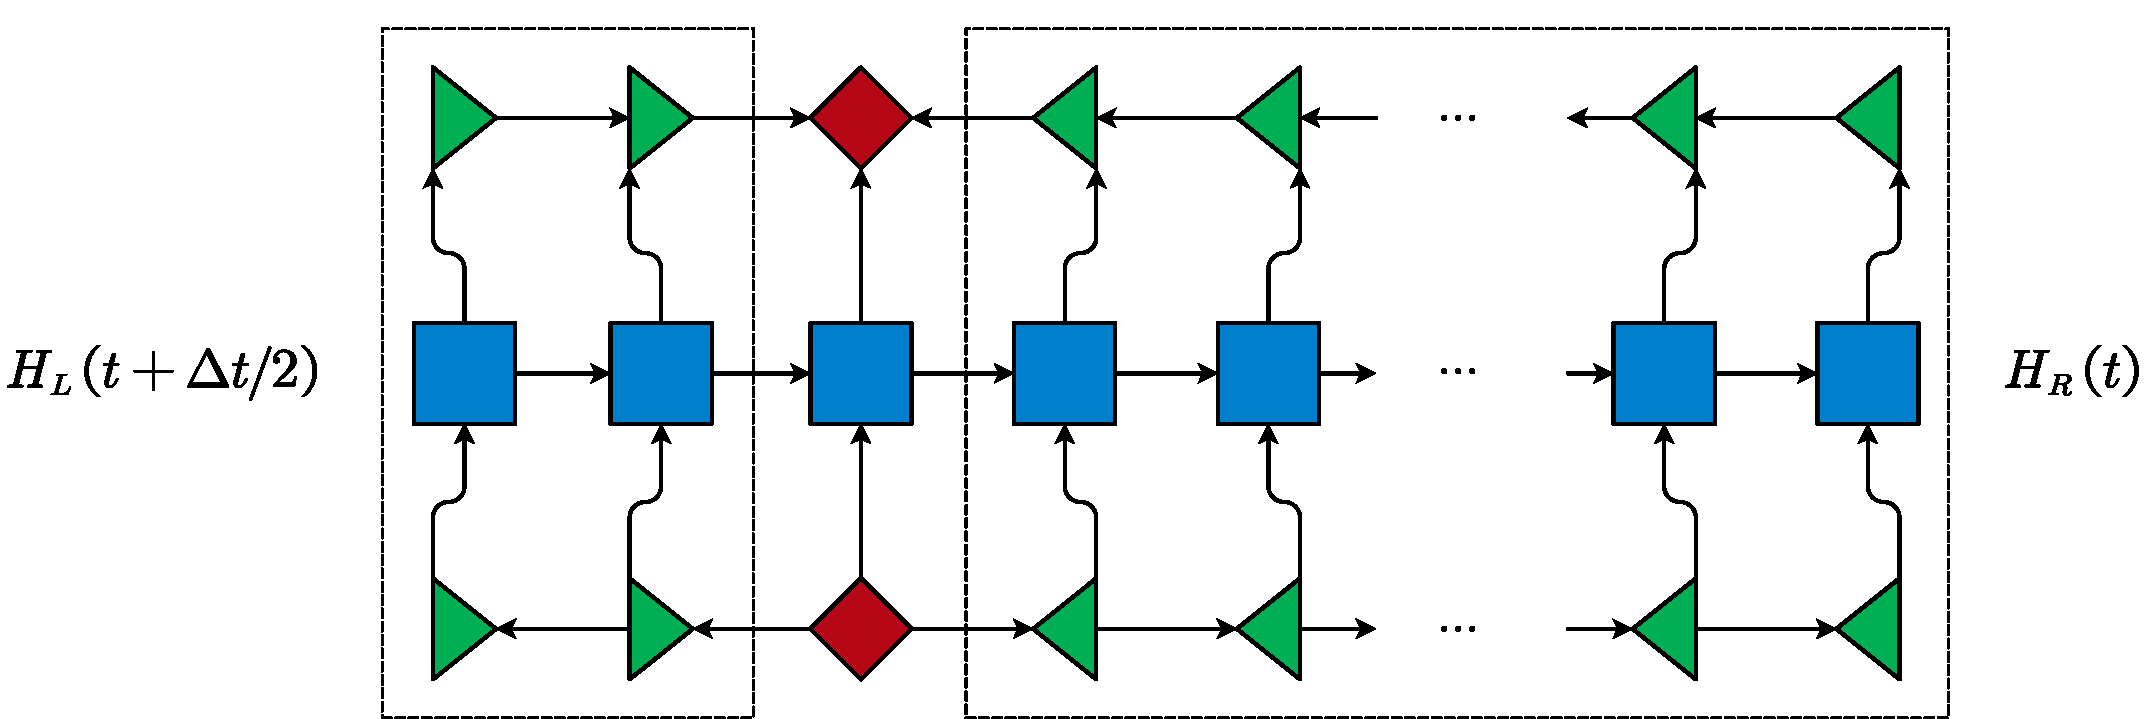
\includegraphics[width=0.8 \linewidth]{images/LRenv1 t.pdf}
			\end{figure}
		\end{itemize}
	\end{itemize}
\end{frame}

\begin{frame}
	\frametitle{Results}
	\setcounter{subfigure}{0}
	Simulation results:
	\begin{figure}[H]
		\centering
		\subfigbottomskip=2pt
		\subfigcapskip=-5pt
		\subfigure{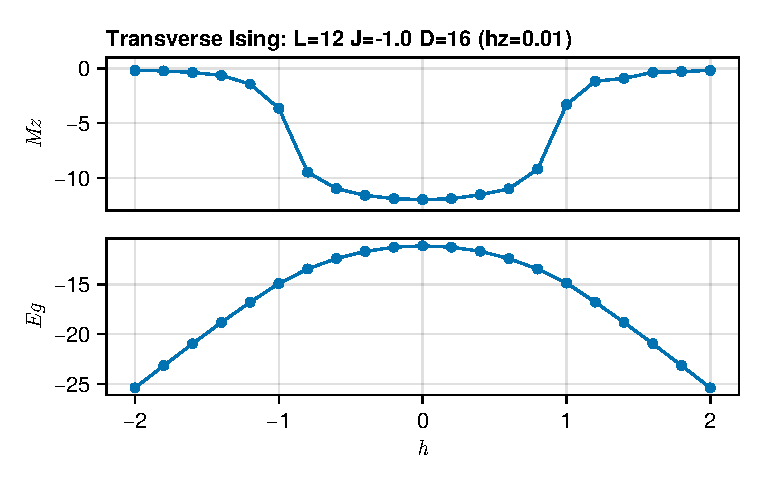
\includegraphics[height=0.31\linewidth]{images/D=16_L=12_J=-1.0.pdf}}
		\subfigure{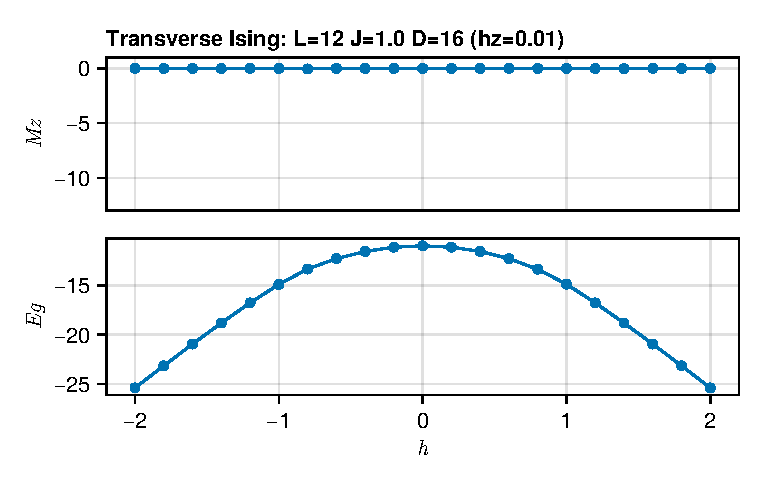
\includegraphics[height=0.31\linewidth]{images/D=16_L=12_J=1.0.pdf}}
	\end{figure}
	a quantum phase transition can be observed near $h\sim 1.0$
\end{frame}

\begin{frame}
	\frametitle{TDVP: 1-site integration}
	\begin{itemize}
		\item Sweep at two direction (right - left - right - \dots)
		\begin{itemize}
			\item Calculate the effective Hamiltonian $H_{eff}^{(1)}$
			\item Time evolution $A_i(t+\Delta t/2) = \exp(-iH_{eff}^{(1)}\Delta t / 2)A_i(t)$ 
			\item OrientSVD and calculate the center with inverse evolution $C_i(t) = \exp(iH_{eff}^{(0)}\Delta t /2) C_i(t+\Delta t/2)$, then absorb it into nextsite.
			\setcounter{subfigure}{0}
			\begin{figure}[H]
				\centering
				\subfigbottomskip=2pt
				\subfigcapskip=-5pt
				\subfigure{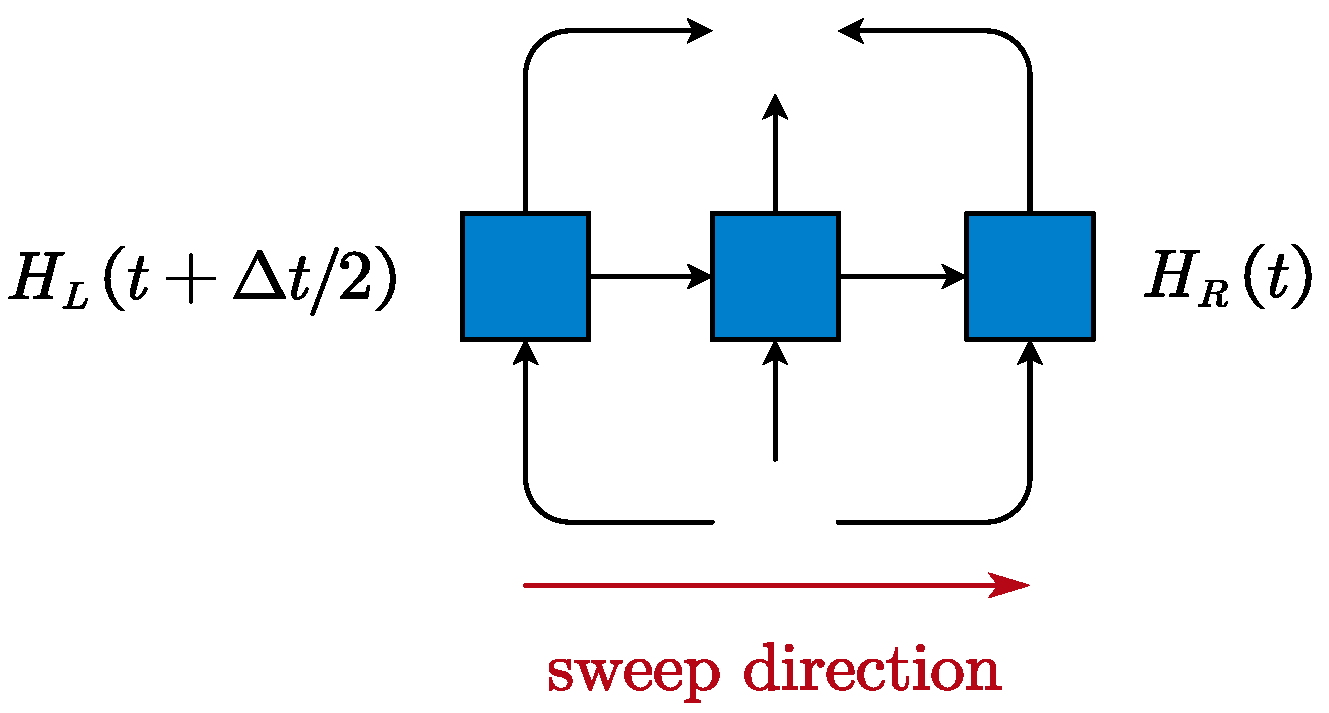
\includegraphics[height=0.2\linewidth]{images/effH1 t.pdf}}
				\subfigure{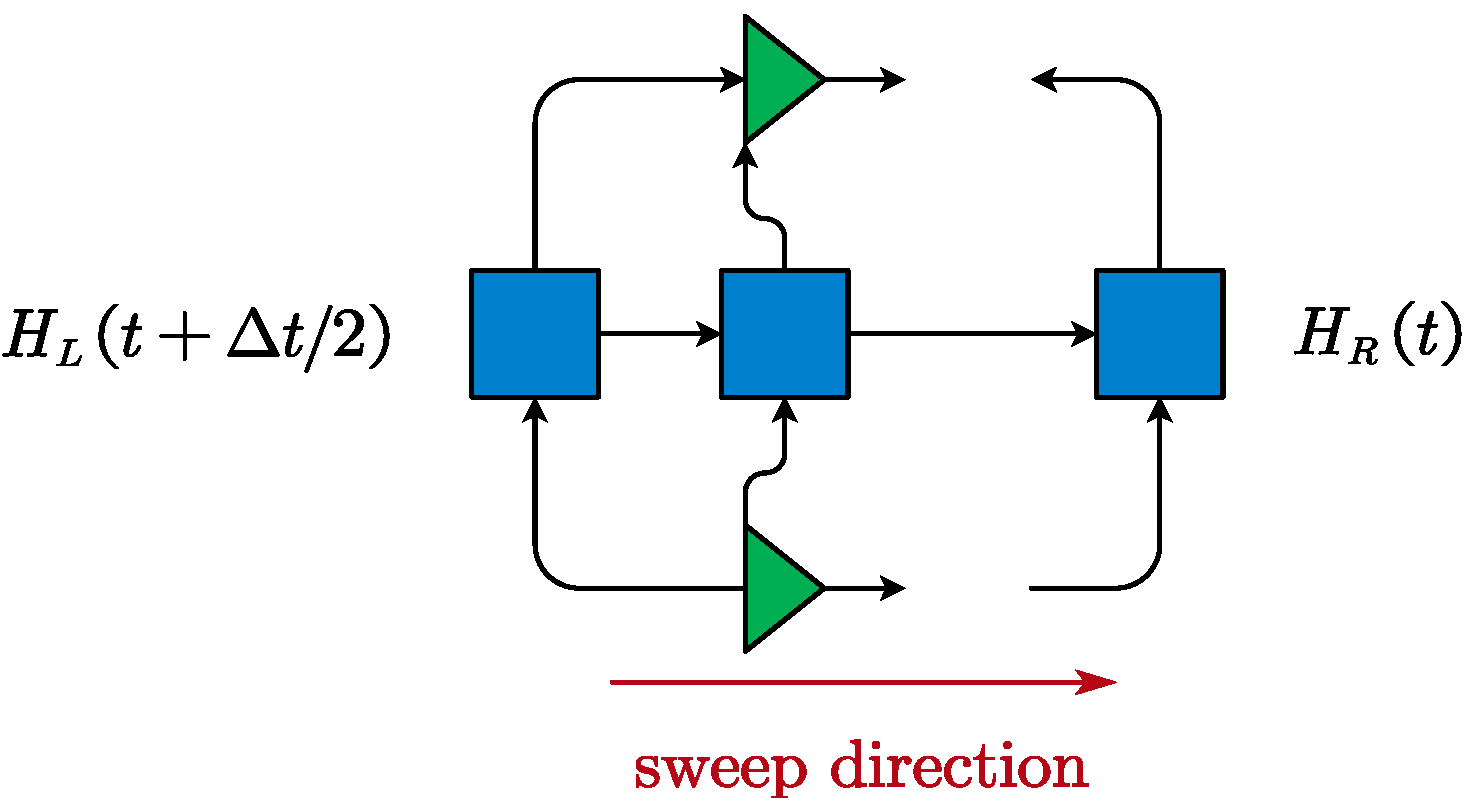
\includegraphics[height=0.21\linewidth]{images/effH0 t.pdf}}
			\end{figure}
		\end{itemize}
	\end{itemize}
\end{frame}

\begin{frame}
	\frametitle{TDVP: 2-site integration}
	Sweep schemes
	\begin{itemize}
		\item Calculate the left/right environment $H_L(t+\Delta t/2)/H_R(t)$.
		\begin{figure}[H]
			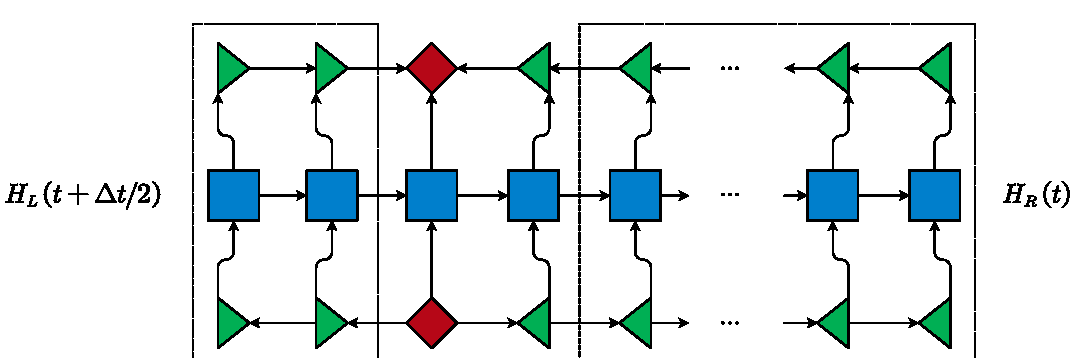
\includegraphics[width=0.8 \linewidth]{images/LRenv2 t.pdf}
		\end{figure}
	\end{itemize}
\end{frame}

\begin{frame}
	\frametitle{TDVP: 2-site integration}
	Sweep schemes
	\begin{itemize}
		\item Calculate the effective Hamiltonian $H_{eff}^{(2)}$
		\item Time evolution $A_iA_{i+1}(t+\Delta t/2) = \exp(-iH_{eff}^{(2)}\Delta t / 2)A_iA_{i+1}(t)$ 
		\item OrientSVD and calculate the center with inverse evolution $A_{i+1}(t) = \exp(iH_{eff}^{(1)}\Delta t /2) A_{i+1}(t+\Delta t/2)$, then regard it as nextsite.
		\begin{figure}[H]
			\centering
			\subfigbottomskip=2pt
			\subfigcapskip=-5pt
			\subfigure{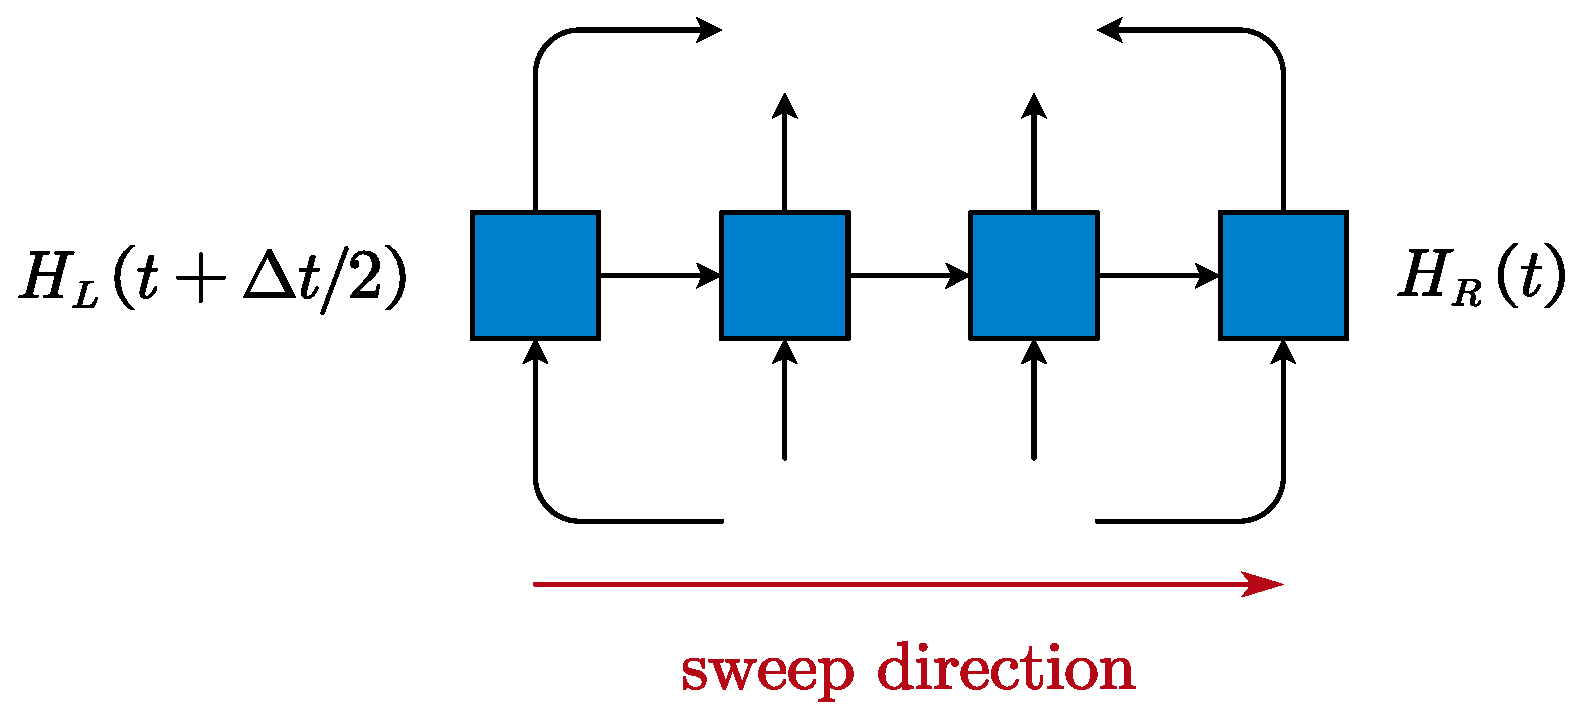
\includegraphics[height=0.2\linewidth]{images/effH2 t.pdf}}
			\subfigure{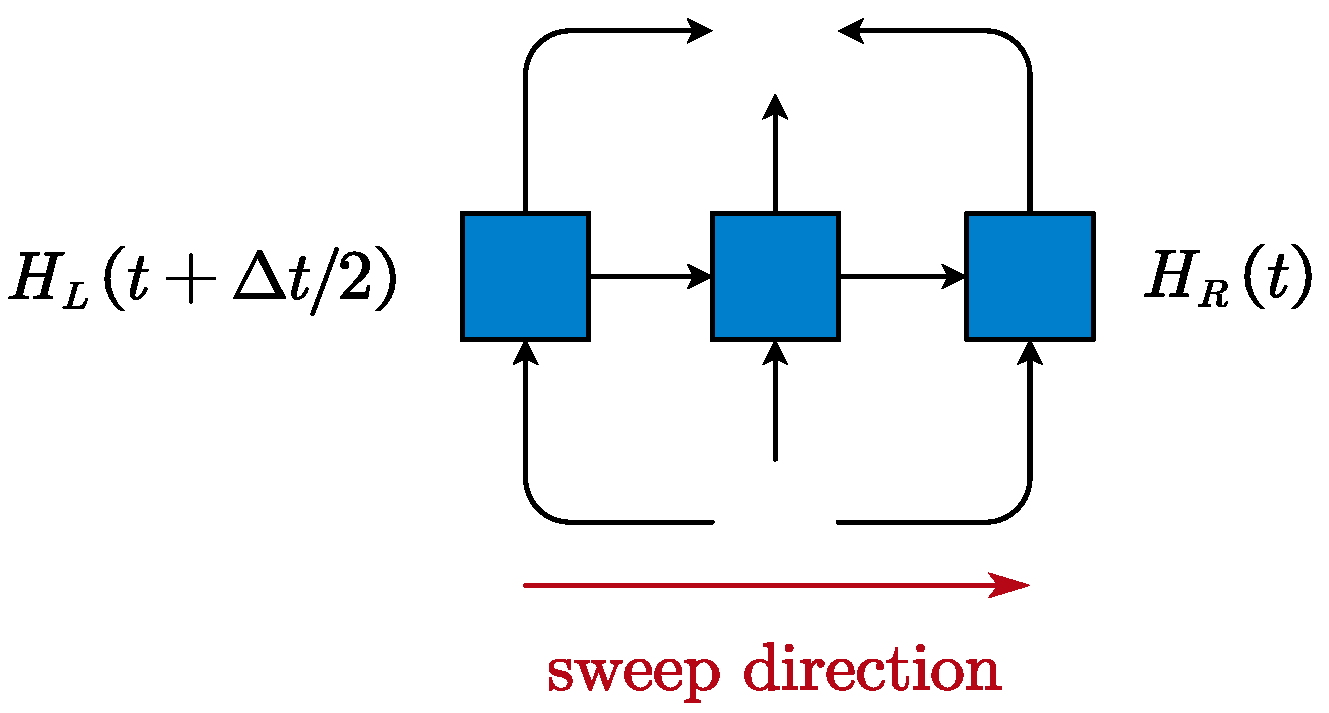
\includegraphics[height=0.2\linewidth]{images/effH1 t.pdf}}
		\end{figure}
	\end{itemize}
\end{frame}

\end{document}
